\documentclass{article}

\usepackage{amsthm}
\usepackage{amsfonts}
\usepackage{amsmath}
\usepackage{amssymb}
\usepackage{fullpage}
\usepackage{graphicx}
\usepackage[usenames]{color}
\usepackage{hyperref}
  \hypersetup{
    colorlinks = true,
    urlcolor = blue,       % color of external links using \href
    linkcolor= blue,       % color of internal links 
    citecolor= blue,       % color of links to bibliography
    filecolor= blue,        % color of file links
    }
    
\usepackage{listings}

\definecolor{dkgreen}{rgb}{0,0.6,0}
\definecolor{gray}{rgb}{0.5,0.5,0.5}
\definecolor{mauve}{rgb}{0.58,0,0.82}

\lstset{frame=tb,
  language=haskell,
  aboveskip=3mm,
  belowskip=3mm,
  showstringspaces=false,
  columns=flexible,
  basicstyle={\small\ttfamily},
  numbers=none,
  numberstyle=\tiny\color{gray},
  keywordstyle=\color{blue},
  commentstyle=\color{dkgreen},
  stringstyle=\color{mauve},
  breaklines=true,
  breakatwhitespace=true,
  tabsize=3
}

\theoremstyle{theorem} 
   \newtheorem{theorem}{Theorem}[section]
   \newtheorem{corollary}[theorem]{Corollary}
   \newtheorem{lemma}[theorem]{Lemma}
   \newtheorem{proposition}[theorem]{Proposition}
\theoremstyle{definition}
   \newtheorem{definition}[theorem]{Definition}
   \newtheorem{example}[theorem]{Example}
\theoremstyle{remark}    
  \newtheorem{remark}[theorem]{Remark}


\title{CPSC-402 Report\\Compiler Construction}
\author{Sebastian Brumm  \\ Chapman University}

\date{\today}

\begin{document}

\maketitle

\begin{abstract}
\end{abstract}

\tableofcontents

\section{Introduction}\label{intro}

\subsubsection{Definitons, Examples, Theorems, Etc}

\section{Homework}\label{homework}

\subsection{Week 1}

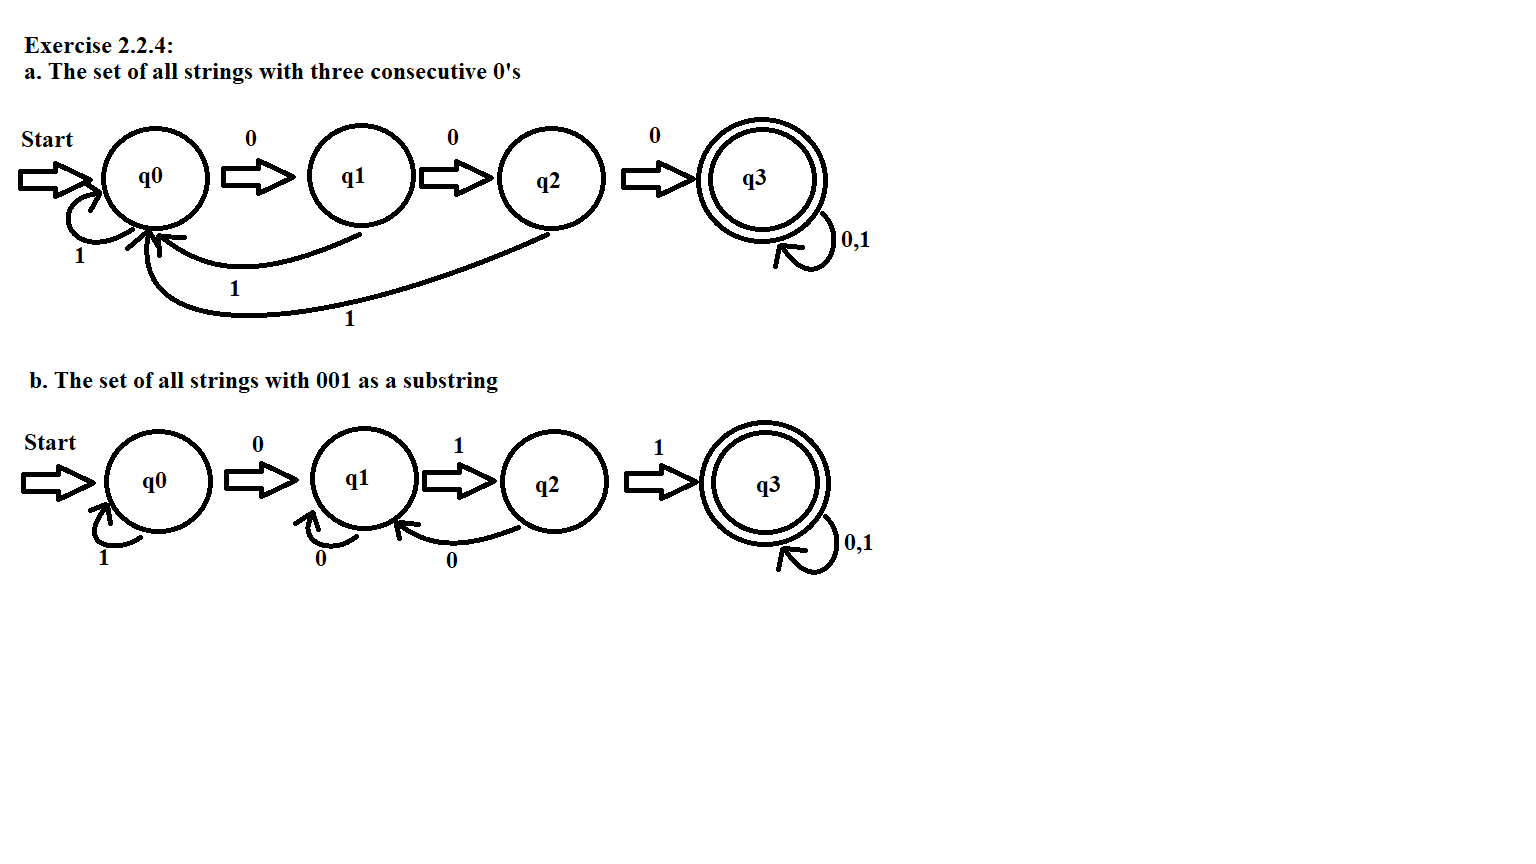
\includegraphics[scale=0.4]{Images/Homework1.png}

\subsection{Week 2}

\subsubsection{2.3.4-a: The set of all strings {0-9} such that the final digit has appeared before}
Regular Expression: $\Sigma^*0\Sigma^*0+...$ add sigma def

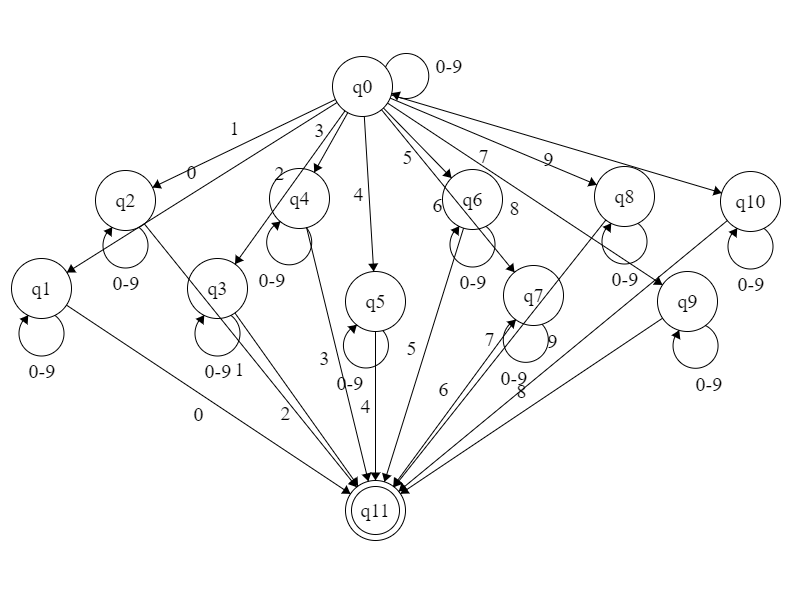
\includegraphics[scale=0.4]{Images/2.3.4a.png}

\subsubsection{2.3.4-b: The set of all strings {0-9} such that the final digit has not appeared before}
Regular Expression: $\{1-9\}0+\{0,2-9\}1...$

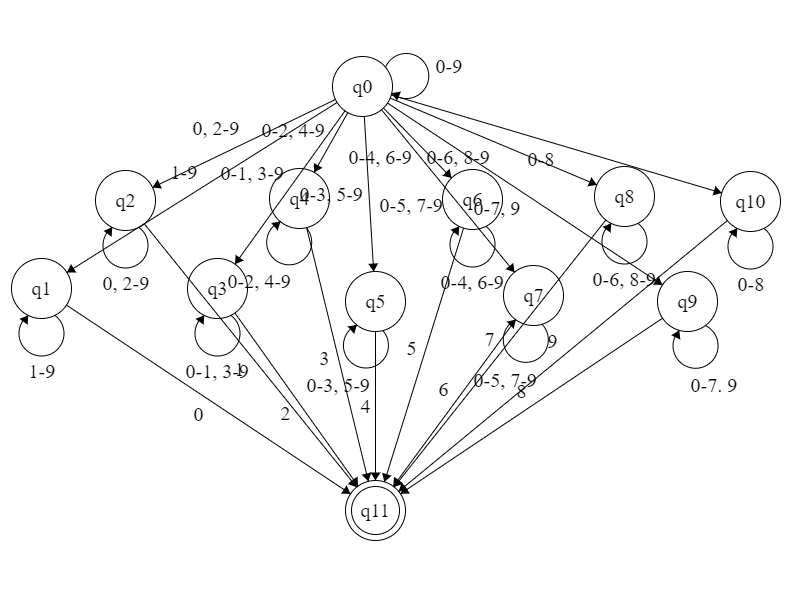
\includegraphics[scale=0.4]{Images/2.3.4b.png}

\subsubsection{2.3.4-c: The set of all strings {0,1} such that there are two 0's separated by a number of positions that is a multiple of 4, including 0}
Regular Expression: $\Sigma^*0\Sigma^{4*}0\Sigma^*$ :wrong automata, add another state after q5 with a zero transition and make it accepting

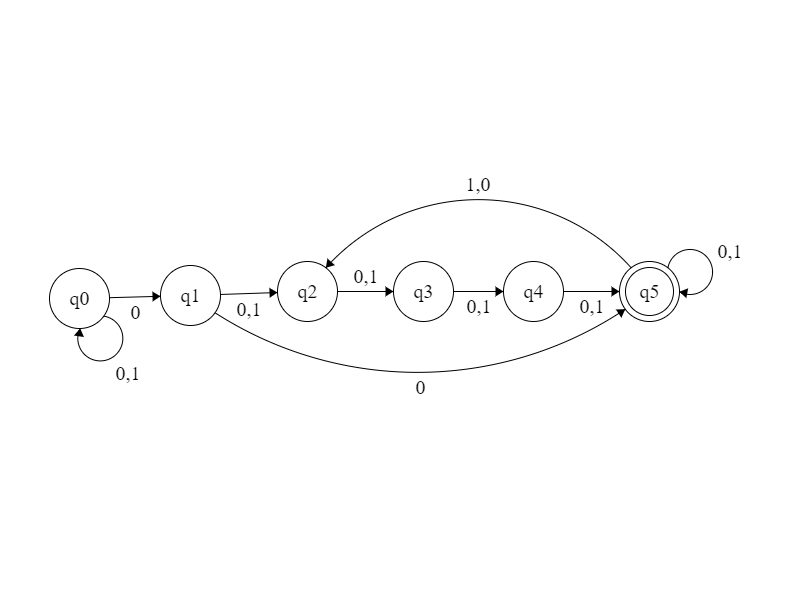
\includegraphics[scale=0.4]{Images/2.3.4c.png}

\subsubsection{2.5.3-a: The set of all strings {a,b,c} consisting of zero or more a's followed by zero or more b's followed by zero or more c's}
Regular Expression: $a^*b^*c^*$

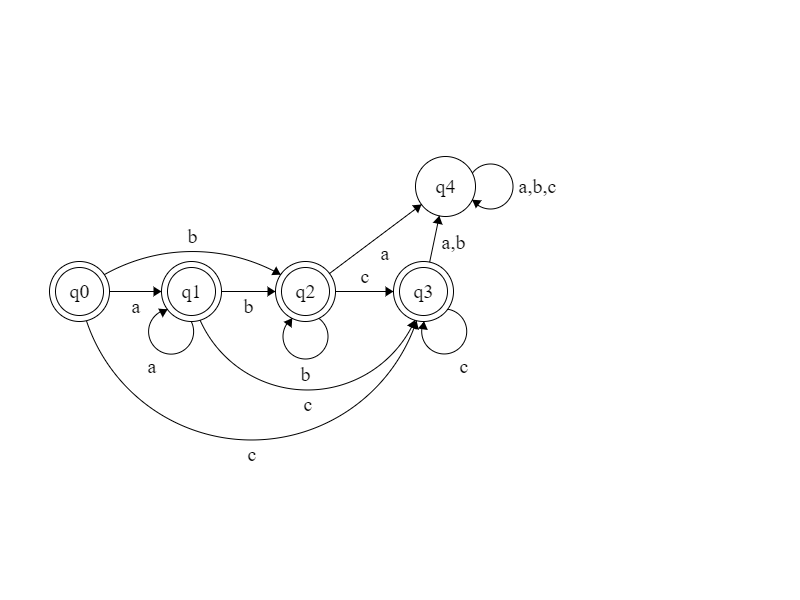
\includegraphics[scale=0.4]{Images/2.5.3a.png}

\subsubsection{2.5.3-b: The set of all strings consisting of either 01 repeated one or more times or 010 repeated one or more times}
Regular Expression: $(01)^++(010)^+$

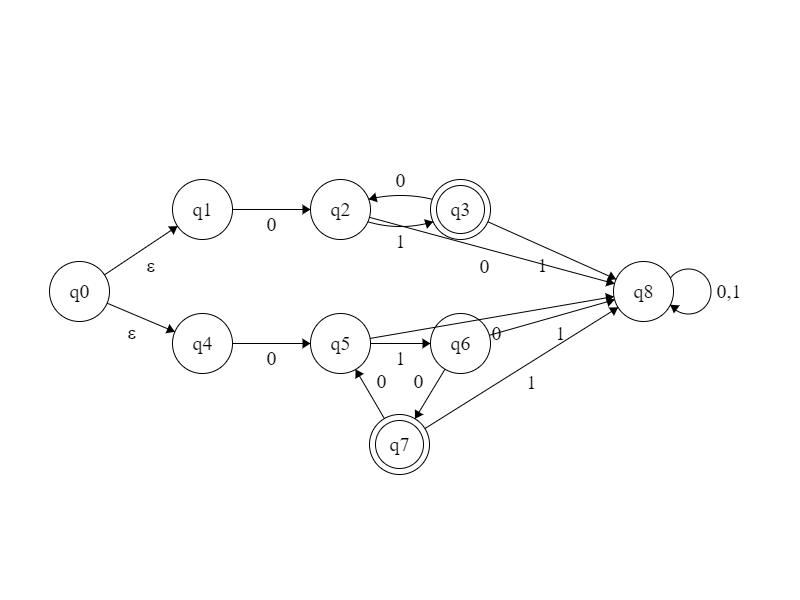
\includegraphics[scale=0.4]{Images/2.5.3b.png}

\subsubsection{2.5.3-c: The set of all strings {0,1} where at least one of the last ten positions is a 1}
Regular Expression: $\Sigma^*1\Sigma^9+\Sigma^*1\Sigma^8...+\Sigma^*1$ : remove loop on the accept state

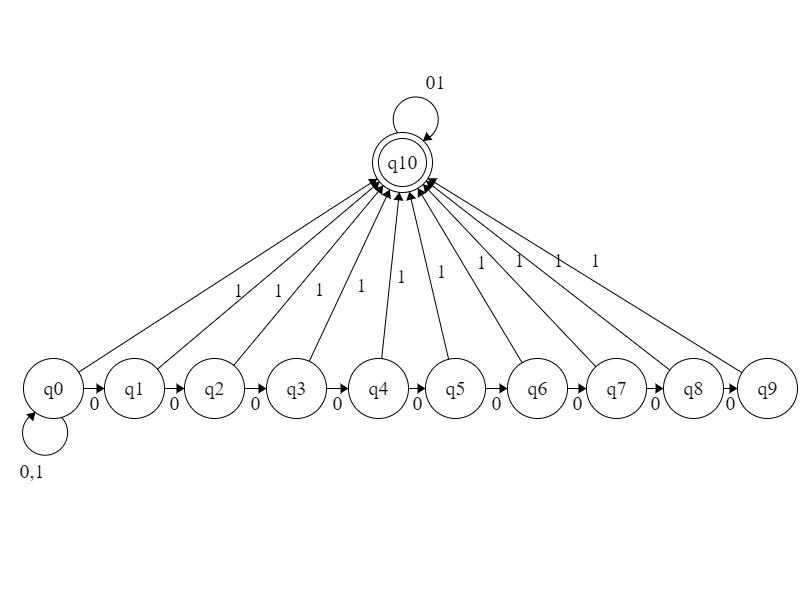
\includegraphics[scale=0.4]{Images/2.5.3c.png}

\subsection{Week 3}

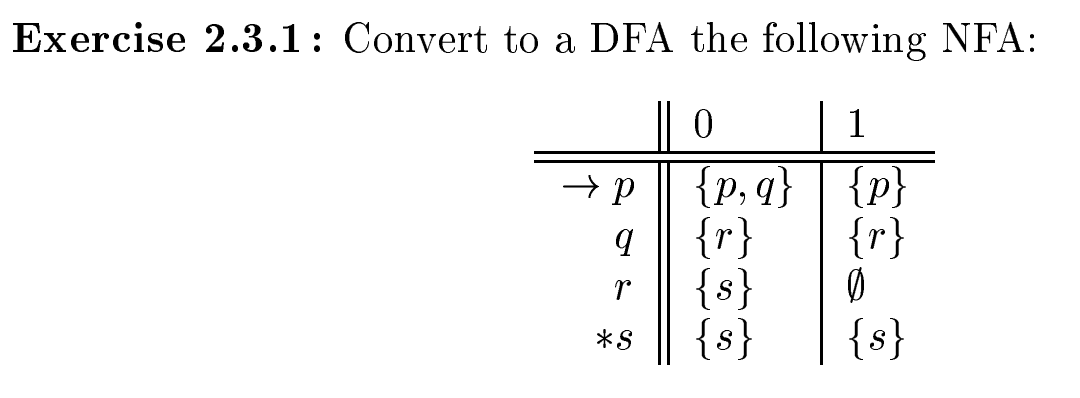
\includegraphics[scale=0.2]{Images/Week3.png}

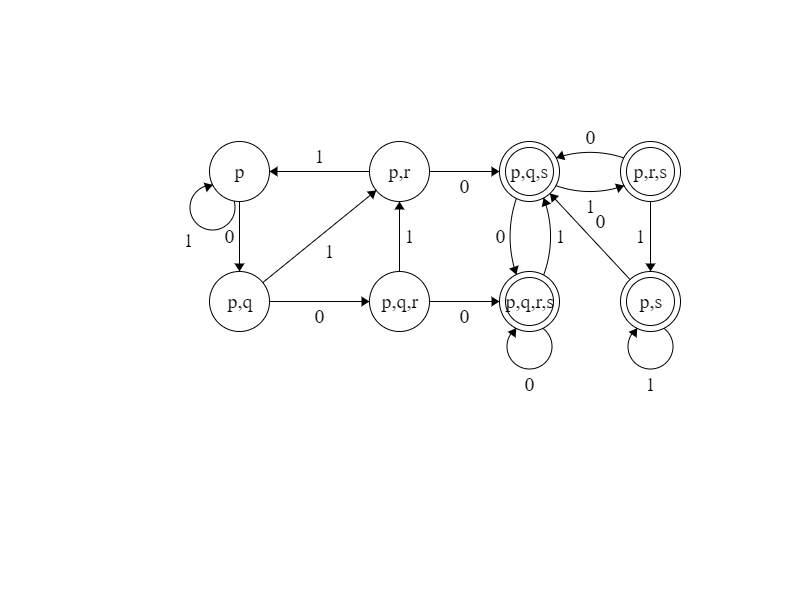
\includegraphics[scale=0.4]{Images/2.3.1.png}

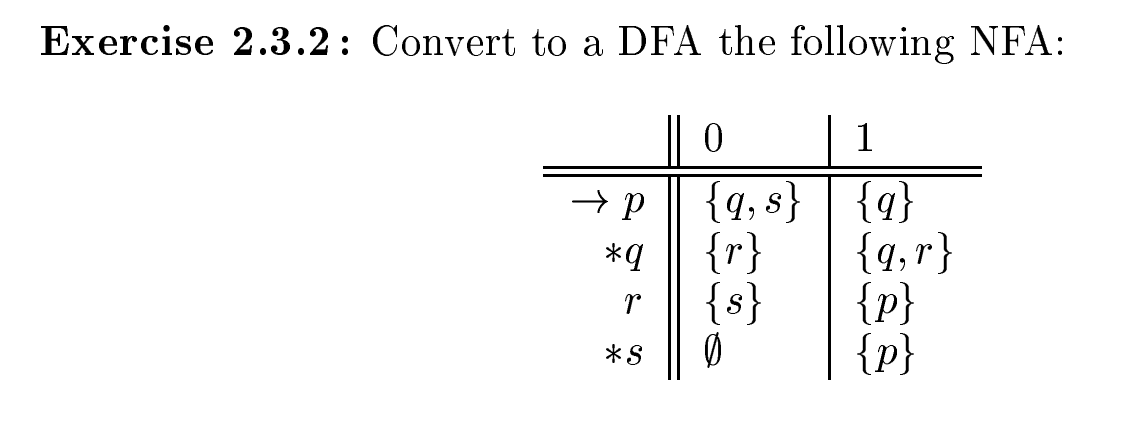
\includegraphics[scale=0.2]{Images/Week3a.png}

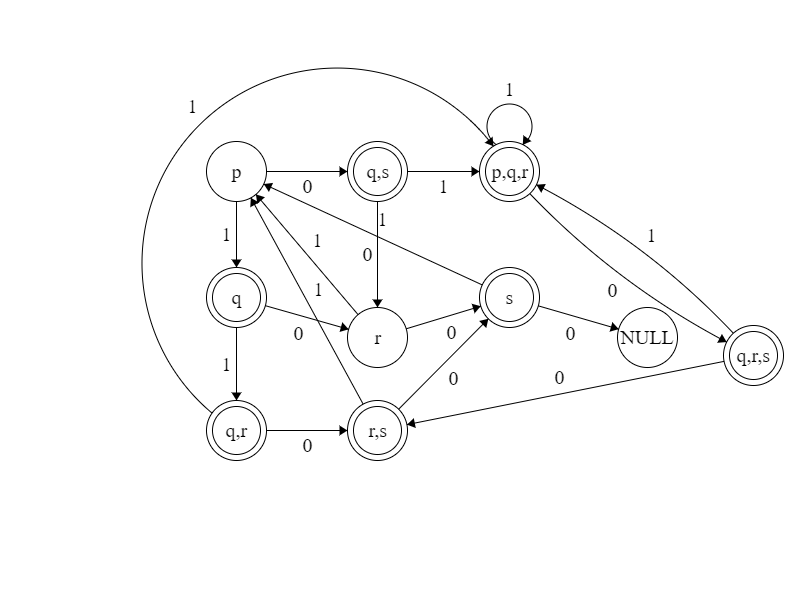
\includegraphics[scale=0.4]{Images/2.3.2.png}

\begin{lstlisting}
-- convert an NFA to a DFA
nfa2dfa :: NFA s -> DFA [s]
nfa2dfa nfa = DFA {
  -- exercise: correct the next three definitions 
  dfa_initial = [(nfa_initial nfa)],
  dfa_final = let
    final qs = disjunction (map (nfa_final nfa) qs)
    in final,
  dfa_delta = let
    delta [] c = []
    delta (q:qs) c = concat [nfa_delta nfa q c, delta qs c]
    in delta }
\end{lstlisting}

The code above is my modifications to the automata05.hs code that converts a non epsilon NFA to a DFA. I have run it with several example strings and have found it to work. The first function dfa\_initial is simple because there are no epsilon transitions here. Therefore, we can simply set the initial state of the NFA to the initial state of the DFA. If there were epsilon transitions, we would also have to account for any possible states that connect to the initial state with an epsilon transition. For the dfa\_final function, we just need to find all states that contain one of the final states from the NFA. This is done using the disjunction and map functions to find if the list of states contains an accepting state. Finally, for the dfa\_delta function, we need to recursively loop through the states that result from an input given the starting state. Both the input and output are a list of states, so we must use the concat function to keep the list as a list of states and not a list of lists.

\section{Project}

\section{Conclusions}\label{conclusions}

\begin{thebibliography}{99}
\bibitem[HMU]{Hopcroft}
	John E. Hopcroft, Rajeev Motwani, Jeffrey D. Ullman:
\href{http://ce.sharif.edu/courses/94-95/1/ce414-2/resources/root/Text\%20Books/Automata/John\%20E.\%20Hopcroft,\%20Rajeev\%20Motwani,\%20Jeffrey\%20D.\%20Ullman-Introduction\%20to\%20Automata\%20Theory,\%20Languages,\%20and\%20Computations-Prentice\%20Hall\%20(2006).pdf}{Introduction to automata theory, languages, and computation,} 3rd Edition. Pearson international edition, Addison-Wesley 2007

\end{thebibliography}

\end{document}
